\documentclass[12pt, letterpaper]{report}
\usepackage[margin=1in]{geometry}
\usepackage[utf8]{inputenc}
\usepackage{graphicx}
\usepackage{amsmath}
\usepackage{float}
\usepackage{subfig}
\graphicspath{ {./img/} }
\setlength\parindent{0pt}
\renewcommand\thesection{\Roman{section}.}
\renewcommand{\thesubsection}{\alph{subsection}.}


\title{CS1675 - Assignment 3}
\author{Zachary M. Mattis}


\begin{document}
	
\maketitle

\section{Problem 1 - Bernoulli Trials}

% A
\subsection{ML Estimate}

\[ \hat{\theta}(x) =  0.65 \]

% B
\subsection{$Beta(\theta | 1,1)$}

\begin{figure}[H]
	\centering
	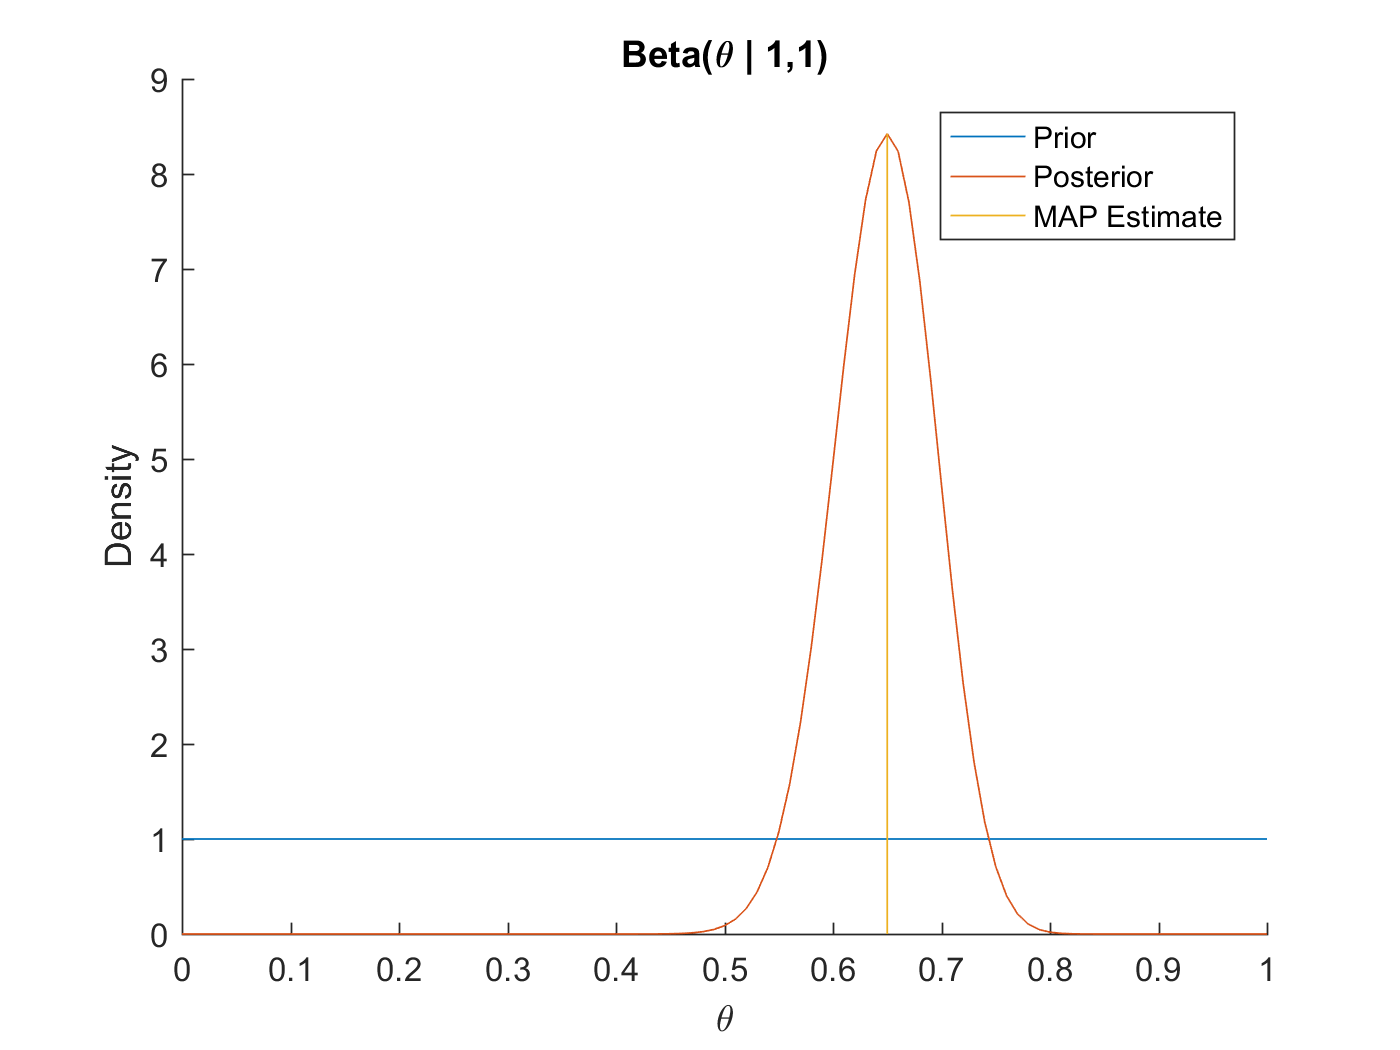
\includegraphics[width=0.7\columnwidth]{p1b.png}
	\caption{Prior = 1,1}
\end{figure}

% C
\subsection{MAP Estimate}


\[ \textrm{MAP Estimate of } \theta = 0.65 \]


% D
\subsection{$Beta(\theta | 4,2)$}

\begin{figure}[H]
	\centering
	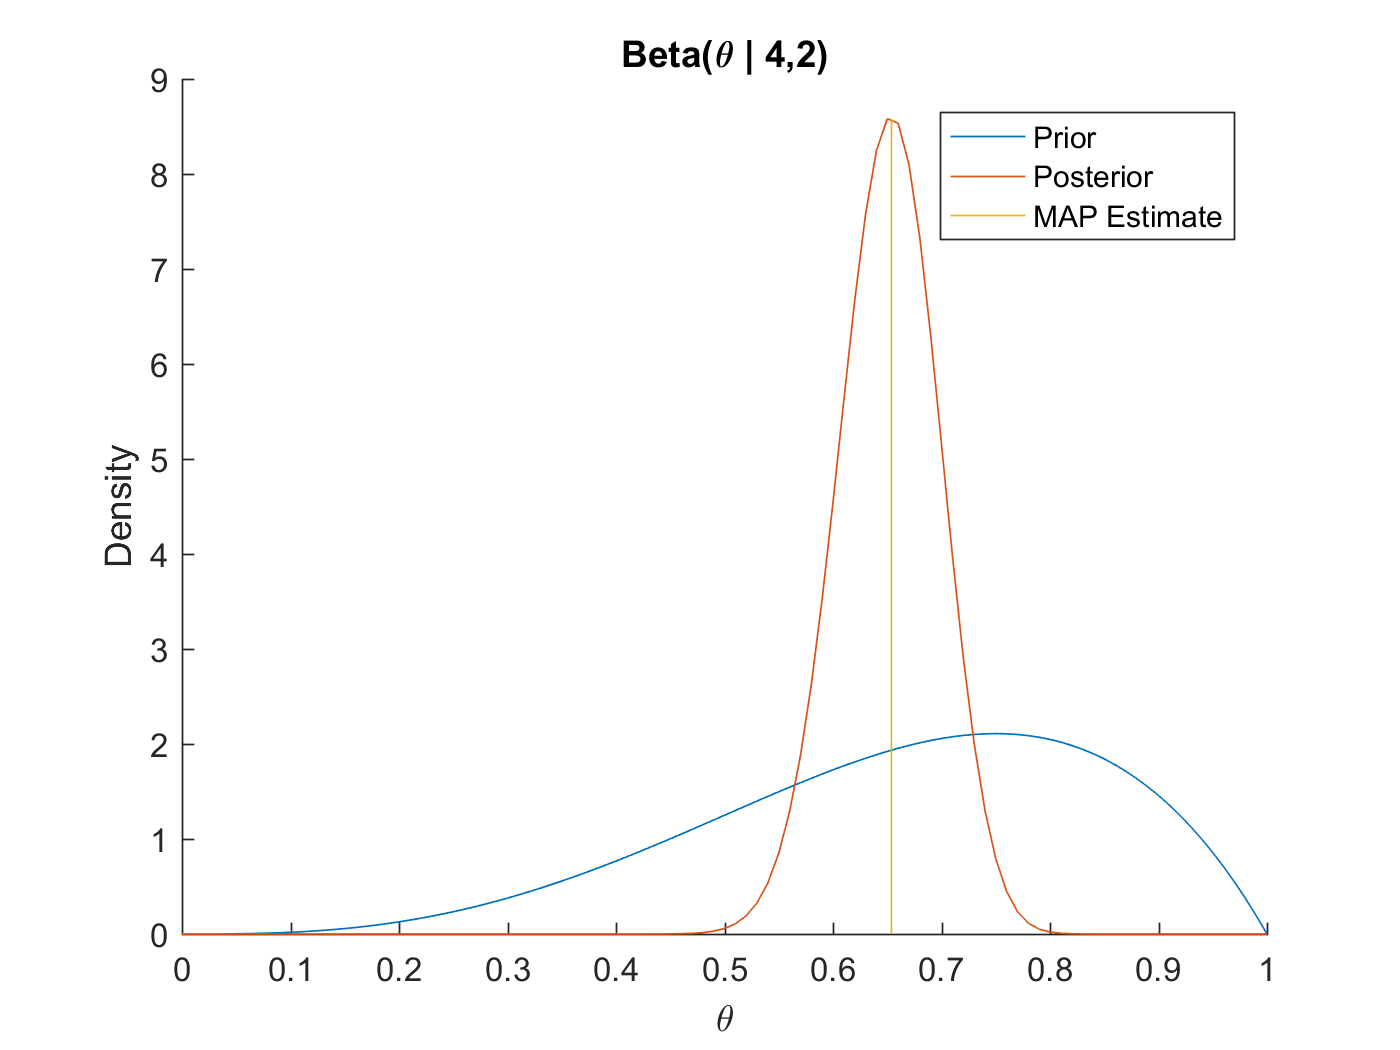
\includegraphics[width=0.7\columnwidth]{p1d.png}
	\caption{Prior = 4,2}
\end{figure}

\[ \textrm{MAP Estimate of } \theta = 0.6538 \]

\section{Problem 2 - Multivariate Gaussian}

% A
\subsection{Gaussian Scatter Plot}

\begin{figure}[H]
	\centering
	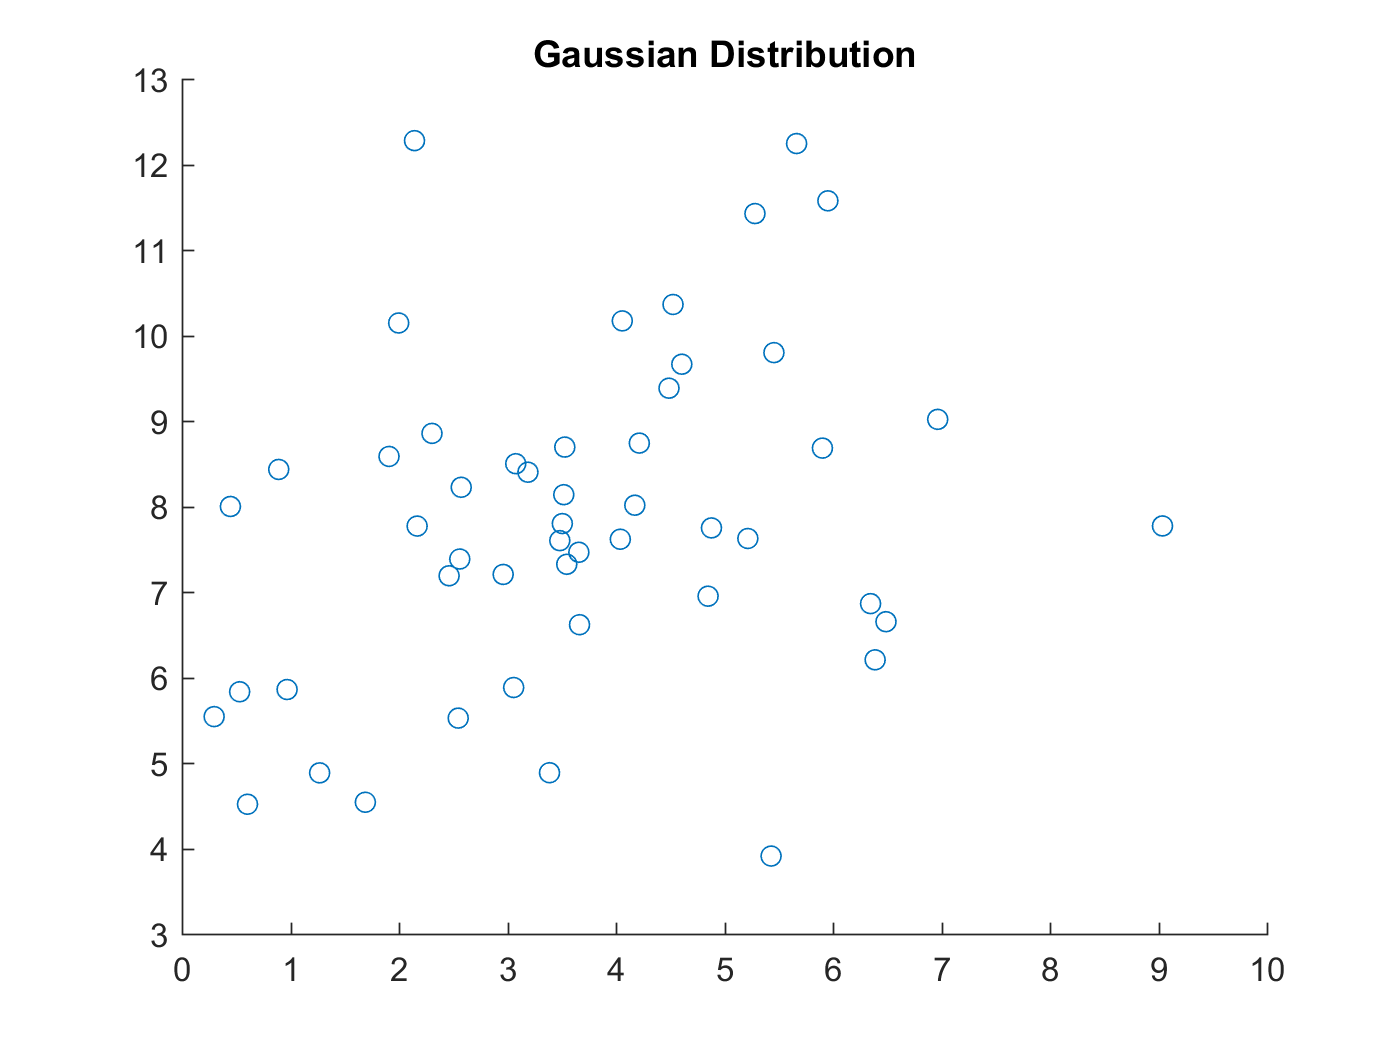
\includegraphics[width=0.7\columnwidth]{p2a.png}
	\caption{Gaussian Scatter Plot}
\end{figure}

% B
\subsection{ML Estimation}

\begin{table}[H]
	\centering
	\begin{tabular}{ |l|l| }
		\hline
		3.6377 & 7.8506 \\
		\hline
	\end{tabular}
	\caption{Mean}
\end{table}

\begin{table}[H]
	\centering
	\begin{tabular}{ |l|l| }
		\hline
		3.6414 & 1.0779 \\
		\hline
		1.0779 & 3.7831 \\
		\hline
	\end{tabular}
	\caption{Covariance}
\end{table}


\begin{figure}[H]
	\centering
	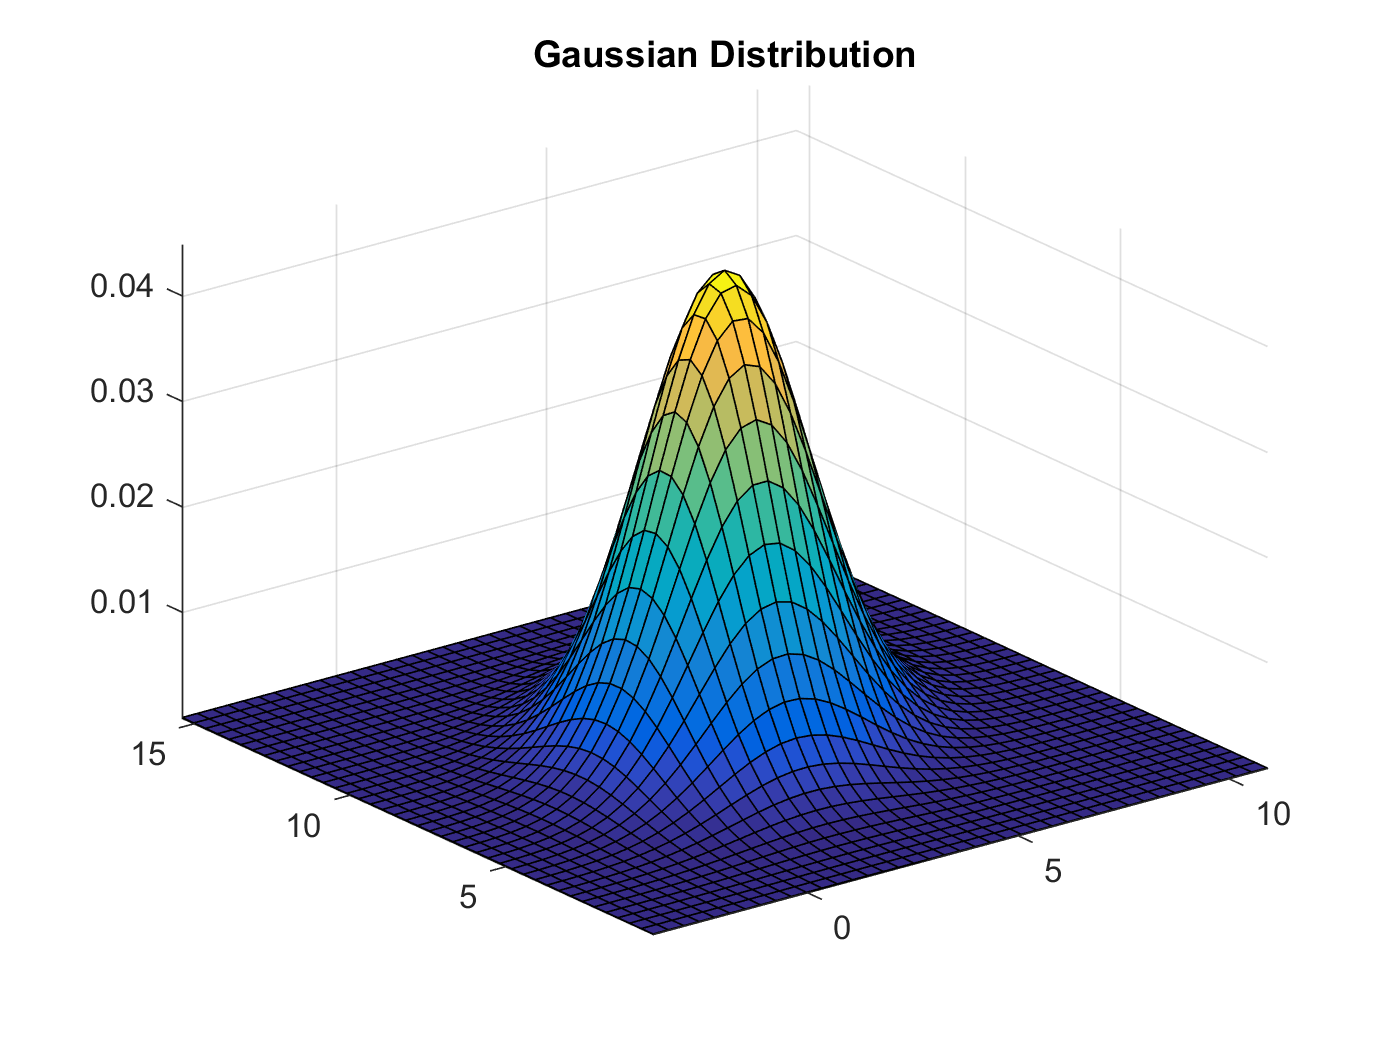
\includegraphics[width=0.7\columnwidth]{p2b.png}
	\caption{Gaussian 3-D}
\end{figure}

% C
\subsection{Individual Gaussian}

\begin{figure}[H]
	\centering
	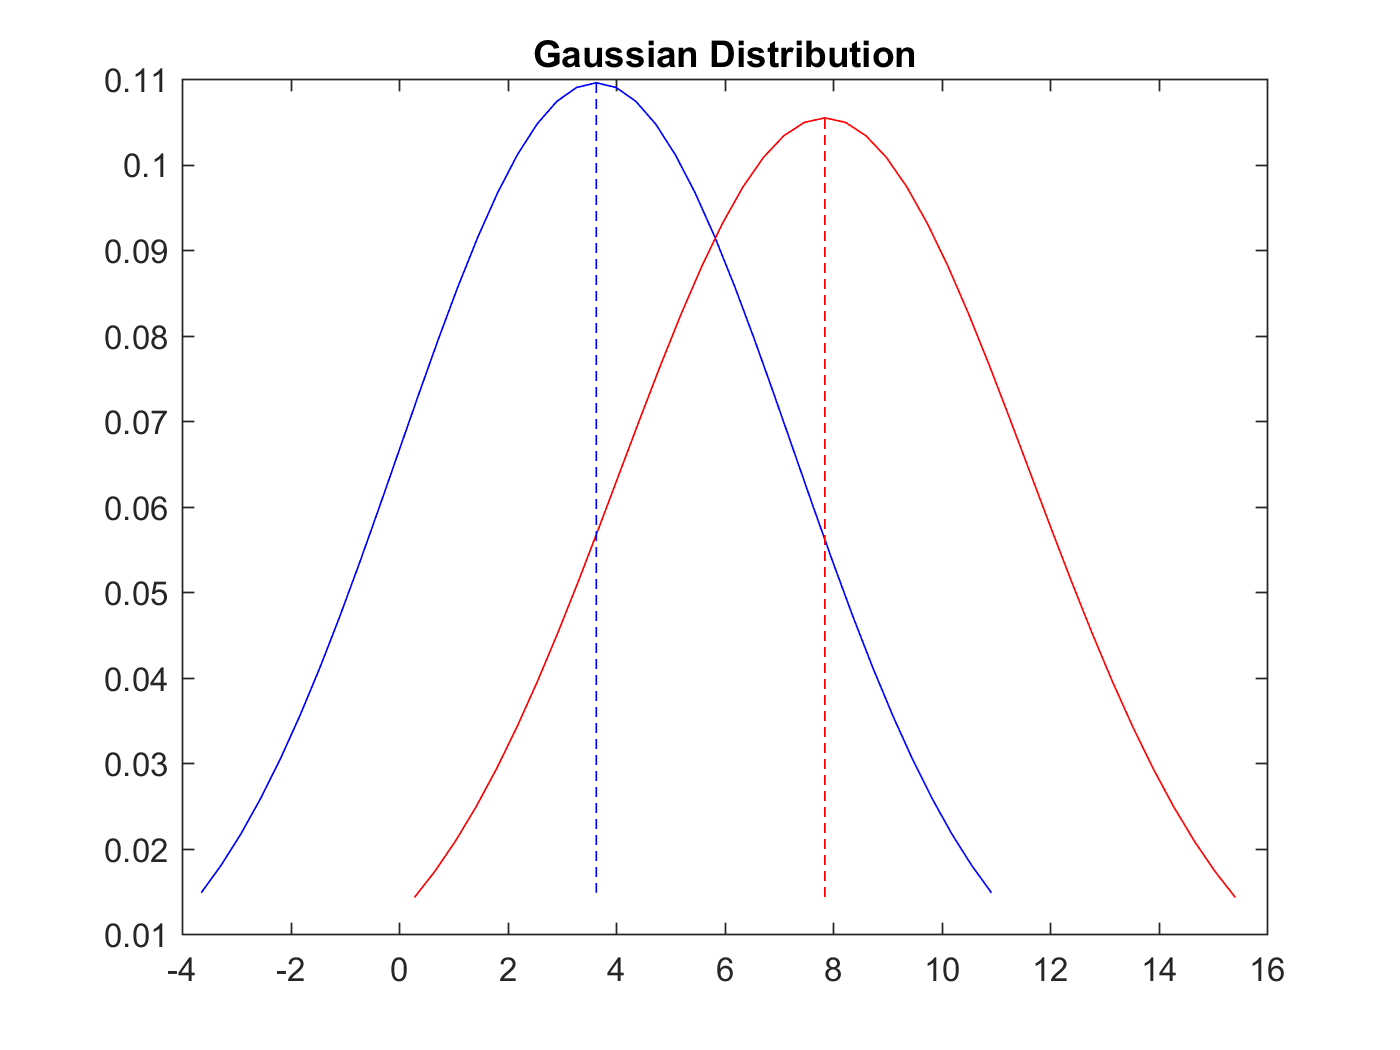
\includegraphics[width=0.7\columnwidth]{p2c.png}
	\caption{Individual Gaussian}
\end{figure}

The first column data of ``gaussian txt" is in blue, while the second is in red.  The corresponding means are 3.6377 and 7.8506.  The corresponding variances are 3.6414 and 3.7831.

% D
\subsection{Multivariate vs. Univariate}

I believe multivariate Gaussian models are a better model than two separate univariate models. Given a multivariate model, it is much easier to view any correlations between the data points as they are directly displayed together. Univariate models need to be interpolated side-by-side and any correlation must be interpreted by the viewer.


\section{Problem 3 - Exponential Distribution}

% A
\subsection{Density Function}

\begin{figure}[H]
	\centering
	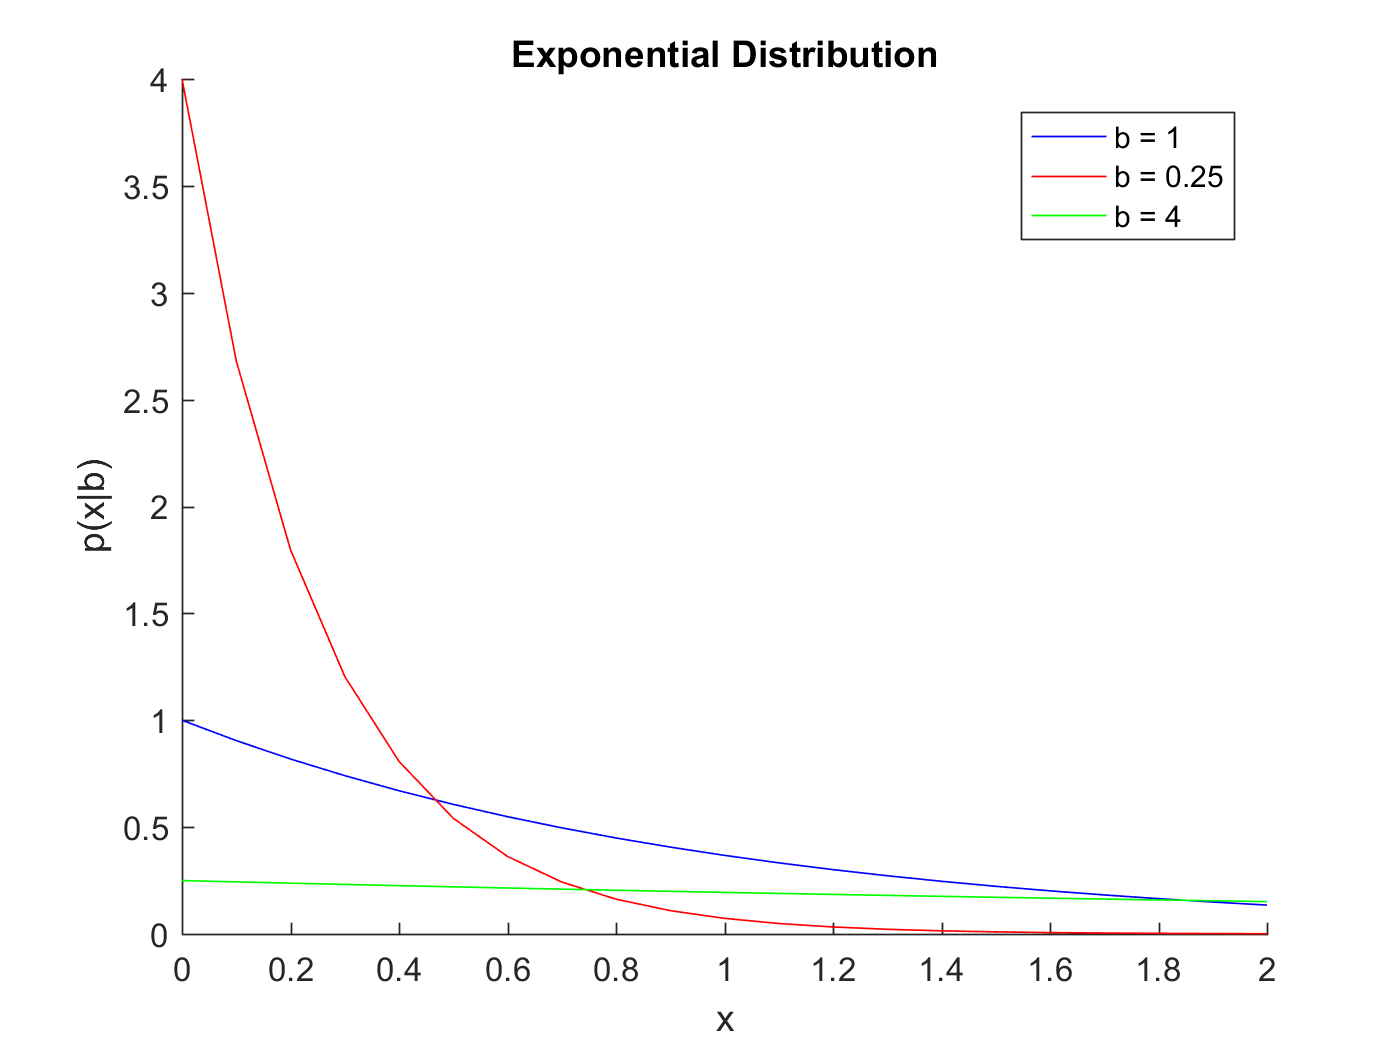
\includegraphics[width=0.7\columnwidth]{p3a.png}
	\caption{Exponential Distribution}
\end{figure}

\subsection{ML Estimate}


\[ f(x;\theta)=\frac{1}{\theta}{e}^{\frac{-x}{\theta}}, 0<x<\infty, \theta\in{[0,\infty}] \]
\\
\[ L(\theta)=L\left(\theta;{x}_{1},{x}_{2}...{x}_{n} \right)=\left(\frac{1}{\theta}{e}^{\frac{{-x}_{1}}{\theta}}\right)\left(\frac{1}{\theta}{e}^{\frac{{-x}_{2}}{\theta}}\right)...\left(\frac{1}{\theta}{e}^{\frac{{-x}_{n}}{\theta}} \right)=\frac{1}{{\theta}^{n}}exp\left(\frac{-\sum_{1}^{n}{x}_{i}}{\theta} \right) \]
\\
\[lnL\left(\theta\right)=-\left(n \right)ln\left(\theta\right) -\frac{1}{\theta}\sum_{1}^{n}{x}_{i}, 0<\theta<\infty\]
\\
\[\frac{d\left[lnL\left(\theta\right) \right]}{d\theta}=\frac{-\left(n \right)}{\left(\theta\right)} +\frac{1}{{\theta}^{2}}\sum_{1}^{n}{x}_{i}=0\]
\\
\[\theta=\frac{\sum_{1}^{n}{x}_{i}}{n}x`\]
\\
\[\Theta=\frac{\sum_{1}^{n}{X}_{i}}{n}\]


\end{document}          